\documentclass{beamer}
\usepackage{polski}
\usepackage[utf8]{inputenc}
\setbeamercovered{transparent}
\author{Marcin TORGiren Fabrykowski}
\title{Wprowadzenie do VIMa}
\institute{AGH - University of Science and Technology}
\usetheme{Frankfurt}
\begin{document}
\begin{frame}
	\titlepage
\end{frame}
\begin{frame}
	\frametitle{O czym będziemy mówić...}
	\tableofcontents
\end{frame}

\section{Co to jest VIM?}
\begin{frame}
	\frametitle{Co to jest?}
	\begin{itemize}[<+->]
		\item Czym jest VIM?
		\begin{block}{Vim}
			Edytor tekstu
		\end{block}
		\item A co z Officem?
		\begin{block}{... Office}
			Procesor tekstu
		\end{block}
	\end{itemize}
\end{frame}

\section[Podstawy podstaw]{Podstawy podstaw - czyli od której strony podejść do VIMa}
\subsection{Wejście i wyjście z VIMa}
\begin{frame}
	\frametitle{Wejście i wyjście z VIMa}
	\begin{itemize}
		\item<1-> Jak włączyć VIMa?
		\begin{block}{Włączenie VIMa}<2->
		vim
		\end{block}
		\item<3-> Jak wyłączyć VIMa?
		\onslide<4->{ ...ale bez generowania losowego ciągu znaków?}
		\begin{block}{Wyłączenie VIMa}<5->
		:q
		\end{block}
	\end{itemize}

\end{frame}
\subsection{Tryby w VIMie}
\begin{frame}
	\frametitle{Tryby w VIMie}
	\begin{itemize}[<+->]
		\item A co jeśli byśmy chcieli wpisać \textit{:q} do pliku?
		\item Dwa tryby pracy:
			\begin{enumerate}
			\item normalny
			\item wstawiania
			\end{enumerate}
		\item Polecenia działają w trybie normalnym
		\begin{block}{Przejscie do tryby normalnego}
			ESC
		\end{block}
		\item Tryb wprowadzania służy do wprowadzania :)
	\end{itemize}
\end{frame}
\subsection{Podstawowe polecenia}
\begin{frame}
	\frametitle{Podstawy podstaw}
	\begin{description}[<+->]
		\item[ESC] Wyjście z trybu wprowadzania/anulowanie polecenia
		\item[:q / :quit] Wyjście z VIMa
		\item[:w / :write] Zapisanie zmian
		\item[:w plik / :write plik] Zapisanie zmian do \textit{plik}
		\item[:q! / :quit!] Wyjście z VIMa bez zapisywania zmian
		\item[:wq] Zapisanie i wyście
		\item[:o plik / :open plik] Otworzenie pliku \textit{plik}
		\item \begin{block}{Zapobieganie utracie dancyh}
			W przypadku dokonania zmian w pliku, \textit{:q} nie pozwoli nam opuścić VIMa. Należy zapisać zmiany - \textit{:w}, bądź wymusić wyjście bez zapisywanie - \textit{:q!}	
			\end{block}
	\end{description}
\end{frame}
\begin{frame}
	\frametitle{Poruszanie się}
	\begin{description}[<+->]
		\item[h,j,k,l] Poruszanie kursorem
		\item[/test] Wyszukiwanie w teksie frazy \textit{test}. Szukanie w przód
		\item[?test] Wyszukiwanie w tekscie frazy \textit{test}. Szukanie wstecz
		\item[n] Przejście do kolejnego wystąpienia szukanej frazy
		\item[w] Przejście na początek kolejnego słowa
		\item[e] Przejście na koniec kolejnego słowa
		\item[b] Przejście na początek poprzedniego słowa
		\item[\textasciicircum] Przejście na początek linii
		\item[\$] Przejście na koniec linii
		\item[gg] Przejście na początek pliku
		\item[G] Przejście na koniec pliku
		\item[u] Undo, cofnięcie zmian
		\item[ctrl+r] Redo, cofnięcie cofnięcia :P	
	\end{description}
\end{frame}
\begin{frame}
	\frametitle{Wstawianie}
	\begin{description}[<+->]
	\item[i] Wstawianie przed kursorem
	\item[a] Wstawianie po kursorze
	\item[o] Wstawianie nowej linii poniżej aktualnej
	\item[O] Wstawianie nowej linii powyżej aktualnej
	\item[I] Wstawianie na początku linii
	\item[A] Wstawianie na końcu linii
	\item[R] Wejście w tryb zastępowania
	\end{description}
\end{frame}
\begin{frame}
	\frametitle{Usuwanie}
	\begin{description}[<+->]
		\item[dd] Usunięcie linii
		\item[dw] Usunięcie wyrazu od kursora do jego końca
		\item[db] Usunięcie wyrazu od jego początku do kursora
		\item[d\$] Usunięcie od kursora do końca linii
		\item[d\textasciicircum] Usunięcie od początku linii do kursora
		\item[dh] Usunięcie znaku na lewo od kursora
		\item[dl] Usunięcie znaku pod kursorem
		\item[x] Usunięcie znaku pod kursorem
		\item[dgg] Usunięcie od początku pliku do kursora
		\item[dG] Usunięcie od kursora do końca pliku
	\end{description}
\end{frame}
\begin{frame}
	\frametitle{Zastępowanie}
	\begin{description}[<+->]
		\item[cw] Usunięcie od kursora do końca wyrazu i przejście w tryb wstawiania
		\item[cb] ...
		\item[c\$] Usunięcie do kursora do końca linii i przejście w tryb wprowadzania
		\item[c\textasciicircum] ...
		\item[cgg] ...
		\item[cG] ...
	\end{description}
\end{frame}
\subsection{Podsumowanie}
\begin{frame}
	\frametitle{Podsumowanie}
	\begin{enumerate}
		\item [ESC] Przejście do trybu normalnego
		\item [i] Przejście do trybu wprowadzania
		\item [:w plik] Zapisanie zmian do pliku \textit{plik}
		\item [:q] Wyjście z VIMa
		\item [A] Dopisywanie na końcu lini
		\item [u] Cofnięcie ostatniej akcji
	\end{enumerate}
\end{frame}
\section{Podstawy VIMa - czyli za co go lubimy}
\subsection{Kolorowanie składni}
\begin{frame}
	\frametitle{Kolorowanie składni - czyli widzimy co mamy zanim to przeczytamy}
	\uncover<1->
	{
		VIM potrafi kolorować składnię.
	}
	\uncover<2->
	{
		\begin{block}{włączenie}
		:syntax on
		\end{block}
	}
	\uncover<3->
	{
		\begin{block}{wyłączenie}
		:syntax off
		\end{block}
	}
	\uncover<4->
	{
		Czy to jest jakaś różnica?
	}
\end{frame}
\begin{frame}
	\frametitle{Bez kolorowania}
	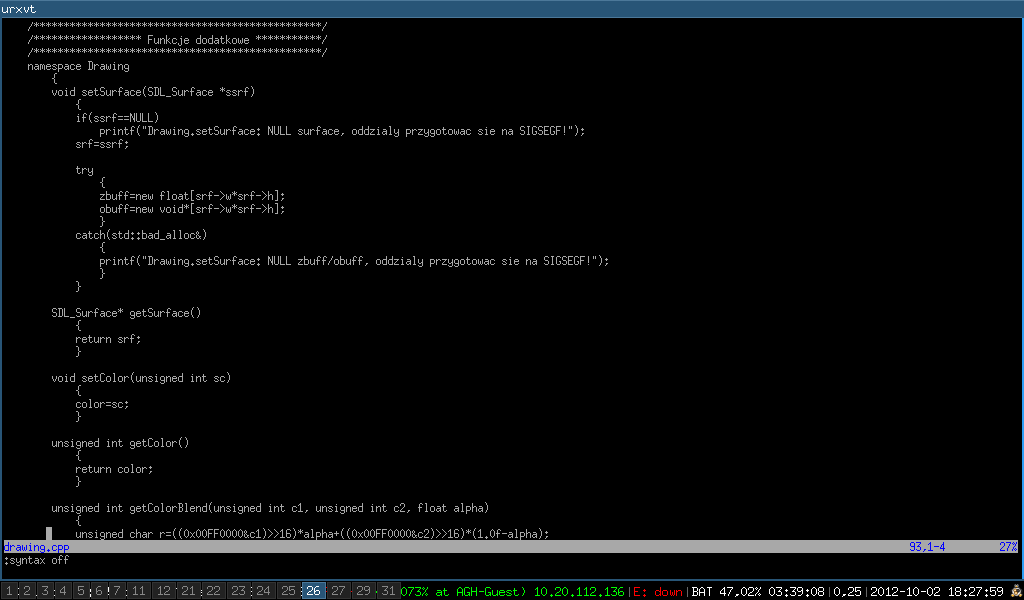
\includegraphics[width=\textwidth]{syntax_off.png}
\end{frame}
\begin{frame}
	\frametitle{z kolorowaniem}
	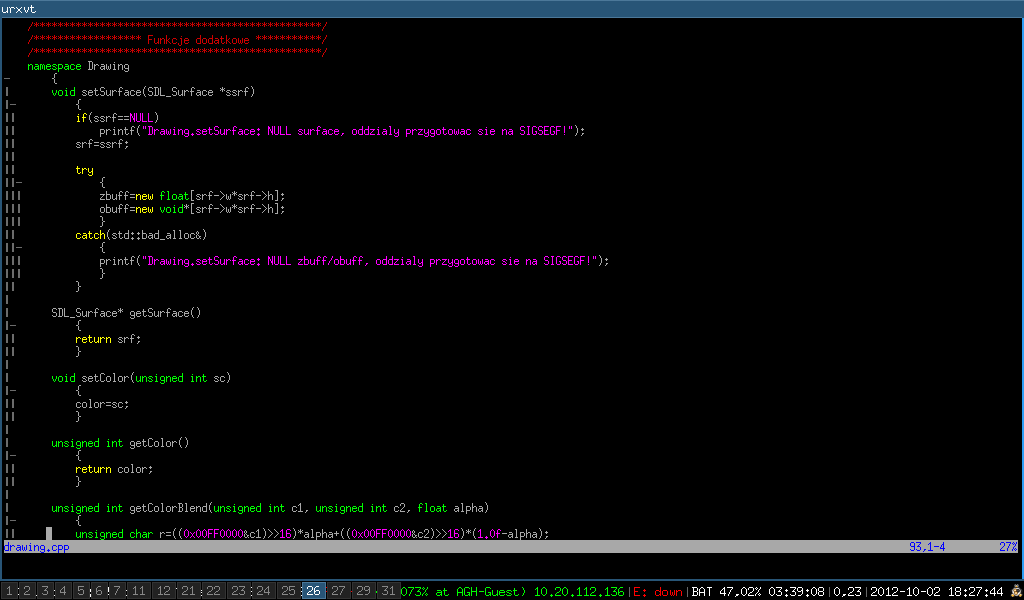
\includegraphics[width=\textwidth]{syntax_on.png}
\end{frame}
\begin{frame}
	\frametitle{Rozpoznawane składnie}
	\begin{enumerate}[<+->]
	\item C/C++
	\item Java
	\item Python
	\item \LaTeX
	\item crontab
	\item fstab
	\item wiele innych...
	\end{enumerate}
\end{frame}
\subsection{Foldowanie - czyli patrzymy tylko po łebkach}
\begin{frame}
	\frametitle{Foldowanie - czyli patrzymy tylko po łebkach}
	\uncover<1->
	{
		Możemy zwijać funkcje, pętle itp\\
	}
	\uncover<2->
	{
		\begin{block}{kiedy zwijamy?}
			Gdy chcemy mieć pogląd całości a nie zagłębiać się w szczegóły
		\end{block}
	}
	\uncover<3->
	{
		Czy jest to potrzebne?
	}
\end{frame}
\begin{frame}
	\frametitle{Metody zwijania - ręczna}
	\begin{block}{włączenie}<1->
	:set foldmethod=manual
	\end{block}
	\begin{block}{tworzenie}<2->
	zf num
	\end{block}
	\begin{block}{usuwanie}<3->
	zd
	\end{block}
	\begin{block}{usuwanie recursywne}<4->
	zD
	\end{block}
	\uncover<5->
	{
		Demonstracja...
	}
\end{frame}
\begin{frame}
	\frametitle{Metody zwijania - markerami}
	\begin{block}{włączenie}<1->
	:set foldmethod=marker
	\end{block}
	\begin{block}{tworzenie}<2->
	\{\{\{ oraz \}\}\}
	\end{block}
	\begin{block}{tworzenie alt.}<3->
	\{\{\{num oraz \}\}\}num
	\end{block}
	\begin{block}{tworzenie alt.2}<4->
	zf num
	\end{block}
	\begin{block}{usuwanie}<5->
	usuwamy znaczniki
	\end{block}
	\begin{block}{usuwanie alt.}<6->
	zd
	\end{block}
	\uncover<7->
	{
		Demonstracja...
	}
\end{frame}
\begin{frame}
	\frametitle{Metody zwijania - wcięcia}
	\begin{block}{włączanie}<1->
	:set foldmethod=indent
	\end{block}
	\begin{block}{tworzenie}<2->
	nie możemy tworzyć
	\end{block}
	\begin{block}{usuwanie}<3->
	nie możemy usuwać
	\end{block}
	\uncover<4->
	{
		Demonstracja...
	}
\end{frame}
\begin{frame}
	\frametitle{Metody zwijania - składnia}
	\begin{block}{włączanie}<1->
	:set foldmethod=syntax
	\end{block}
	\begin{block}{tworzenie}<2->
	nie możemy tworzyć
	\end{block}
	\begin{block}{usuwanie}<3->
	nie możemy usuwać
	\end{block}
	\uncover<4->
	{
		Demonstracja...
	}
\end{frame}
\begin{frame}
	\frametitle{Poruszanie się po foldach}
	\begin{enumerate}[<+->]
		\item [zo] Otwiera zagnieżdżenie
		\item [zO] Otwiera zagnieżdżenie rekursywnie 
		\item [zc] Zamyka zagnieżdżenie
		\item [zC] Zamyka zagnieżdżenie rekursywnie
		\item [zm] Zamyka jeden poziom foldów w pliku
		\item [zM] Zamyka wszystkie foldy
		\item [zr] Otwiera jeden poziom foldów w pliku
		\item [zR] Otwiera wszystkie foldy
	\end{enumerate}
\end{frame}
\begin{frame}
	Dziękuję za uwagę
\end{frame}
\end{document}
